
\begin{frame}{Combinatoire : maîtrise difficile des signaux}
    \begin{block}{Rappel : La logique combinatoire}
        Les sorties ne dépendent que des entrées présentes. Mais en pratique... le temps existe !
    \end{block}

    %\vspace{0.3em}
    \begin{columns}
        \column{0.60\textwidth}
        \textbf{Problématiques physiques :}
        \begin{itemize}
            \item \textbf{Délais de propagation (\(\tau_{pd}\)) :} Les portes mettent du temps à calculer (durée non-déterministe).
            \item \textbf{Aléas (hazards) :} Apparition de transitoires parasites lors de changements simultanés.
        \end{itemize}
        \vspace{0.1em}
        \textbf{Conséquences en cascade :}
        \begin{itemize}
          \item Impossible de prédire exactement \textit{à partir de} \textbf{quand} un signal est stable.
          \item \textbf{Composer} de grands blocs combinatoires mène à un chaos temporel ingérable.
        \end{itemize}
        \begin{alertblock}{Constat}
          La complexité des systèmes explose et la fiabilité s'effondre.
        \end{alertblock}

        \column{0.35\textwidth}
        %\begin{center}
          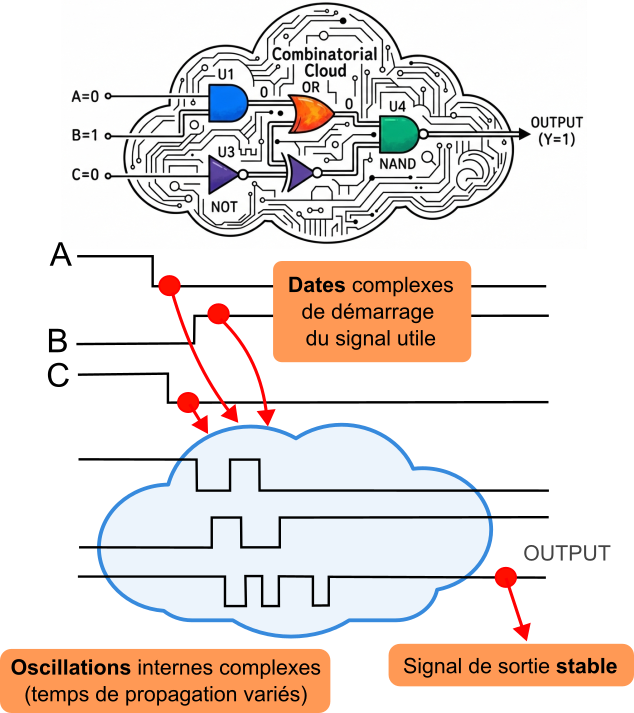
\includegraphics[scale=0.31]{./images/bascule_d_v0.png}
        %\end{center}
    \end{columns}

\end{frame}
%
% \begin{frame}{Combinatoire : maîtrise difficile des signaux}
%   \begin{center}
%     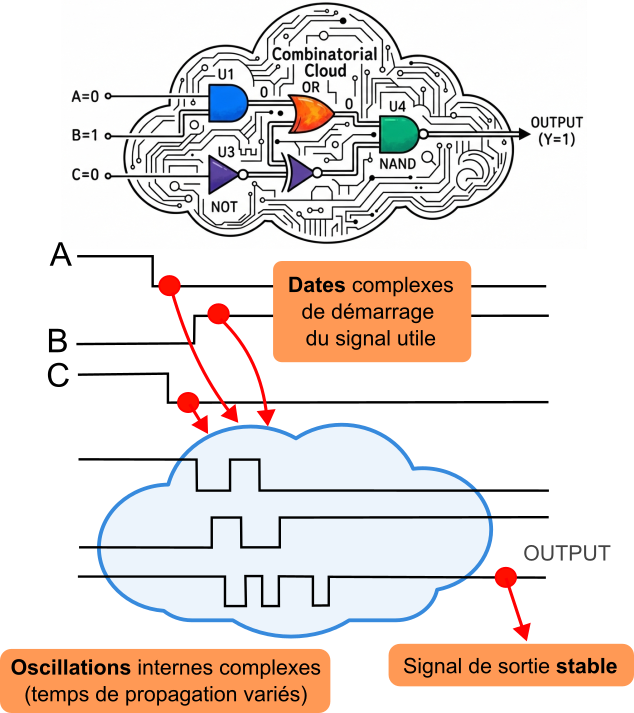
\includegraphics[scale=0.4]{./images/bascule_d_v0.png}
%   \end{center}
% \end{frame}

\begin{frame}{Le système synchrone mono-cadencé : Maîtriser le temps}
    \begin{block}{L'idée directrice}
        Plutôt que de subir les délais continus, on segmente le temps à l'aide d'un \textbf{métronome commun, unique}  : \textbf{l'horloge}. Elle est suffisamment lente pour que tous les signaux se stabilisent avant leur échantillonnage.
    \end{block}

    \vspace{0.3em}
    \begin{itemize}
        \item \textbf{Le quantum de temps :} Le cycle d'horloge (\(T\)) devient l'unique unité de référence.
        \item \textbf{Séparation des rôles :}
        \begin{itemize}
            \item Le \textit{combinatoire} calcule la nouvelle valeur (pendant que le signal se stabilise).
            \item La \fbox{\textit{bascule D}} mémorise cette valeur au moment précis du front d'horloge (montant pour nous).
        \end{itemize}
        \item \textbf{Bénéfice majeur :} On s'affranchit des variations technologiques et des délais intermédiaires ; on ne raisonne plus en nanosecondes, mais en \textbf{coups d'horloge}.
    \end{itemize}

    \vspace{0.5em}
    \begin{exampleblock}{Conclusion}
        La \fbox{bascule D} est la brique de base qui permet de synchroniser le monde et de passer du « temps continu incertain » au « temps discret maîtrisé ».
    \end{exampleblock}
\end{frame}


\begin{frame}{Bascule D : symbole, table de vérité et chronogramme}
  \begin{center}
    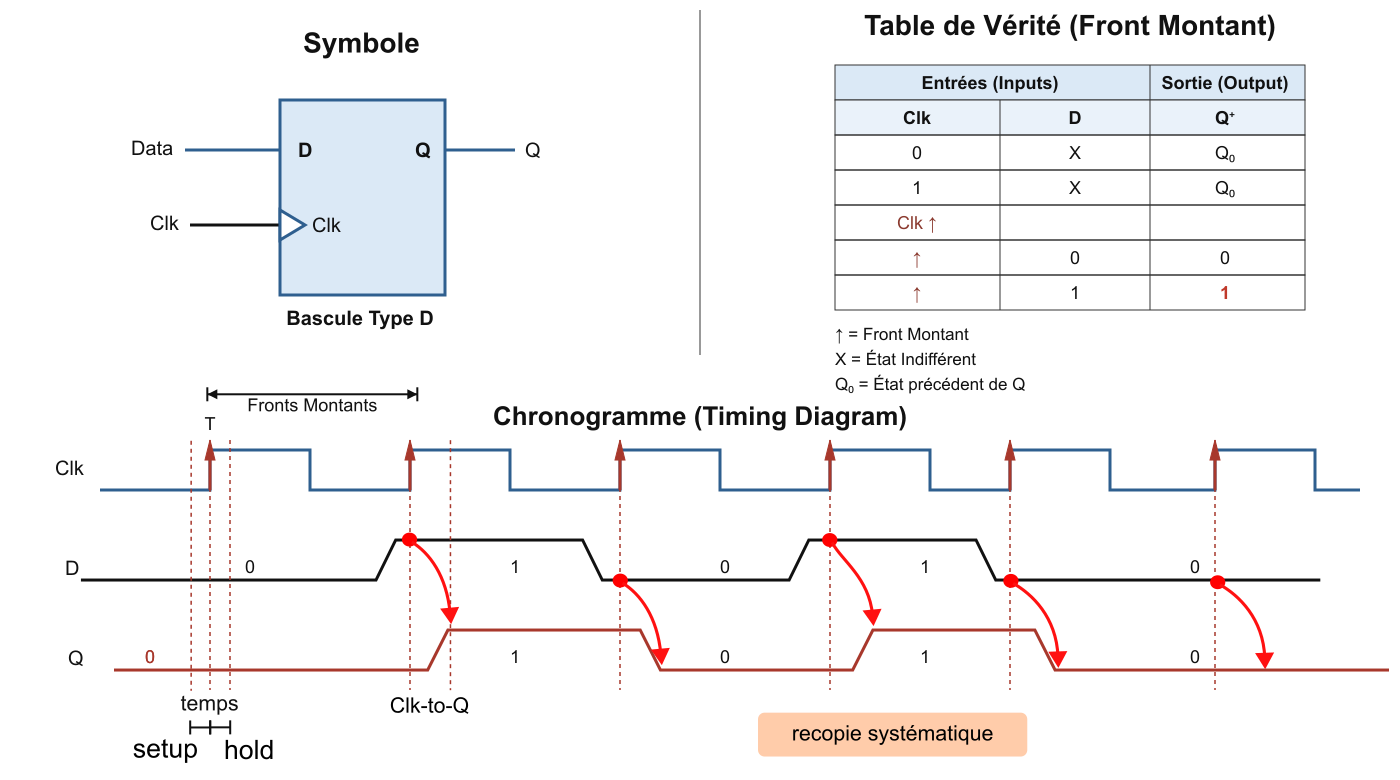
\includegraphics[scale=0.35]{./images/bascule_d.png}
  \end{center}
\end{frame}


\begin{frame}{La bascule D : un décalage d’un cycle d’horloge}
  %\framesubtitle{Du comportement microscopique au point de vue macroscopique}

  \begin{block}{Ce qu’il faut retenir}
    Une bascule D recopie l’entrée \(D\) sur la sortie \(Q\) \textbf{au rythme de l’horloge}.
    \[
      Q_{n+1} = D_n
    \]
    Autrement dit : \alert{\(Q\) est la version de \(D\), retardée d’un cycle }.
  \end{block}

  \vspace{0.1cm}

  \begin{columns}[T]
    \begin{column}{0.48\textwidth}
      \textbf{Vue microscopique (complexe)}
      \begin{itemize}
        \item chronogramme détaillé.
        \item temps de \emph{setup} et de \emph{hold}
        \item recopie exacte après le délai \(t_{\text{Clk}\to Q}\)
        \item phénomènes transitoires
      \end{itemize}

    \end{column}

    \begin{column}{0.48\textwidth}
      \textbf{Vue macroscopique (simple)}
      \begin{itemize}
        \item on oublie les détails temporels fins
        \item on attend que tous les signaux soient stables : $T_{clock} >> \text{max}(\{T_{crit}(f)\},\forall f \in \mathbb{O})$
        \item on ne garde que : \alert{un coup d’horloge = un pas de retard}
      \end{itemize}
    \end{column}
  \end{columns}

  \begin{alertblock}{On bascule dans l’Informatique !}
    La bascule D transforme un signal continu en \textbf{suite numérique}.
  \end{alertblock}
\end{frame}

\begin{frame}{Bascule D : précautions d'utilisation}
  \begin{columns}
    \begin{column}{0.5\textwidth}
      \begin{enumerate}
        \item Le signal \texttt{D} doit être stable \underline{avant} et \underline{après} le front montant.
        \begin{itemize}
          \item temps de \texttt{setup}
          \item temps de \texttt{hold}
        \end{itemize}
        \item Sinon : risque de \textbf{métastabilité}
        \begin{itemize}
          \item tension intermédiaire imprévisible
          \item ...avant stabilisation aléatoire (O ou 1)
          \item ...au bout d'un délai variable
        \end{itemize}
      \end{enumerate}
      \begin{center}
        \includegraphics[scale=0.15]{./images/hill.jpg}
      \end{center}
    \end{column}
    \begin{column}{0.5\textwidth}
      \begin{enumerate}[3]
        \item Le \textbf{passé} du signal \texttt{D} se trouve sur la sortie \texttt{Q}
      \end{enumerate}
      \begin{center}
        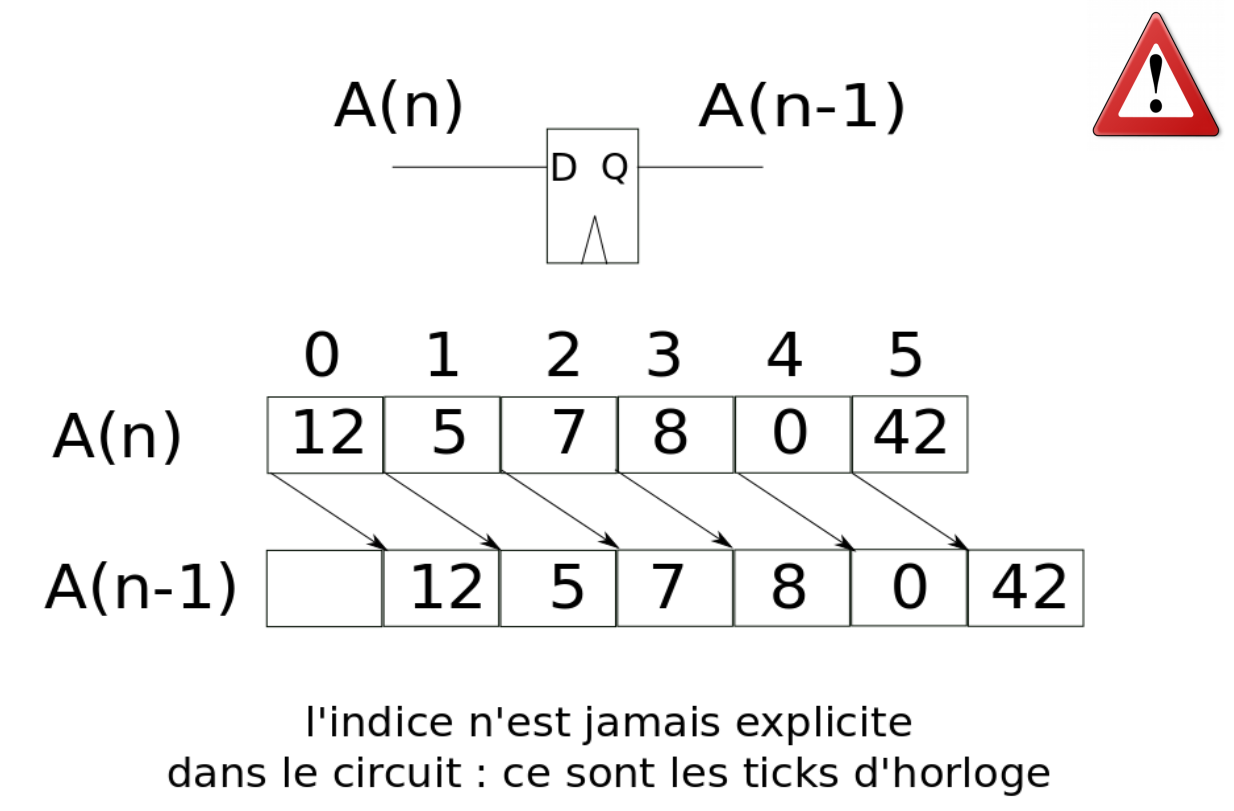
\includegraphics[scale=0.18]{./images/bascule_d_indices.png}
      \end{center}
    \end{column}
  \end{columns}
\end{frame}

\begin{frame}{Bascule D : constitution interne}

  \begin{alertblock}{Attention : \textit{"Ne pas reproduire à la maison"}}
    \begin{itemize}
      \item La règle de \texttt{conception synchrone} \fbox{interdit} les \textbf{cycles combinatoires}.
      \begin{itemize}
        \item Il est difficile \texttt{de savoir} si une boucle stabilise ou pas (ici oui).
        \item Veiller à ne pas introduire de telles boucles de manière subtile.
        \item Ne conservez que la bascule D. Oubliez les autres.
      \end{itemize}
    \end{itemize}
  \end{alertblock}

  \begin{center}
      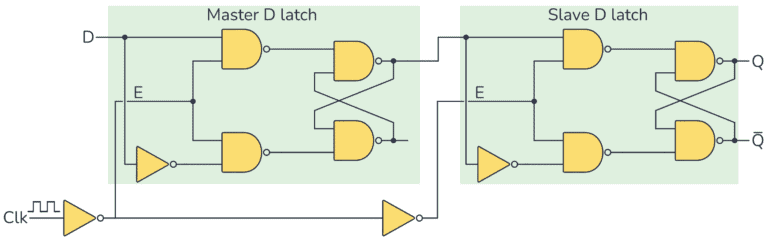
\includegraphics[scale=0.3]{./images/dff.png}
  \end{center}

  \begin{block}{Info}
    Plusieurs structures internes de bascule D. En CMOS notamment : portes de transmission.
  \end{block}
\end{frame}


\begin{frame}{Bascule D : mémorisation par \textit{recirculation} des données}
  \begin{alertblock}{Objectif}
    Comment mémoriser une \underline{même} donnée \textbf{pendant plusieurs cycles} ?
  \end{alertblock}

  \begin{columns}
    \begin{column}{0.5\textwidth}
      \begin{itemize}
        \item \textbf{Rappel} :
        \begin{itemize}
          \item la bascule D mémorise son état durant \underline{une} période d'horloge
          \item un nouveau front $\rightarrow$ échantillonnne une \underline{nouvelle} donnée sur \texttt{D}.
        \end{itemize}
        \item \textbf{Solution : }\fbox{Recirculation} à l'aide d'un \texttt{multiplexeur} \footnote{rappel : le multiplexeur est combinatoire}.
        \begin{enumerate}
          \item Un signal de contrôle (ici \texttt{load}) accompagne la donnée entrante \texttt{A}.
          \item La bascule \texttt{D} ré-échantillonne la donnée capturée, présente sur \texttt{F}, à chaque cycle.
        \end{enumerate}
      \end{itemize}
      % \begin{block}{Note}
      %   Il existe aussi des langages \textit{informatiques} qui utilisent le \textbf{modèle synchrone} : systèmes critiques, avionique,...
      % \end{block}
    \end{column}
    \begin{column}{0.5\textwidth}
      \begin{center}
        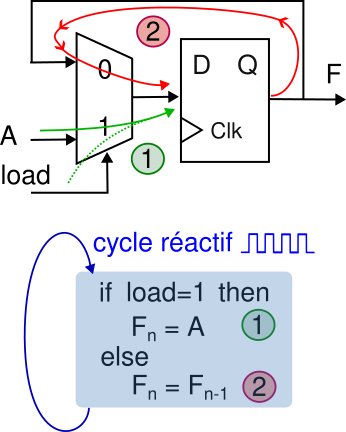
\includegraphics[scale=0.45]{./images/recirculation.png}
      \end{center}
    \end{column}
  \end{columns}
\end{frame}

\begin{frame}{Exemple : analyseur de sourires}
  \begin{columns}
    \begin{column}{0.5\textwidth}
      \begin{center}
        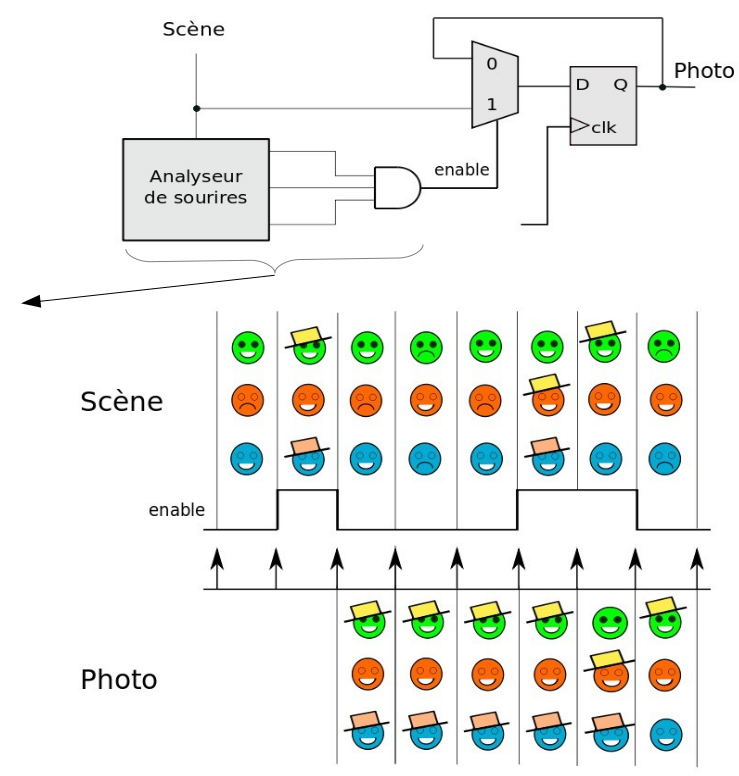
\includegraphics[scale=0.26]{./images/analyseur_sourires.png}
      \end{center}
    \end{column}
    \begin{column}{0.5\textwidth}
      $\leftarrow$ On suppose que l'analyseur est purement combinatoire....\\
      \vspace{0.5cm}
      \textbf{Apparition d'un schéma générique} :
      \begin{alertblock}{On retient :}
        \begin{itemize}
          \item Calculs "verticaux" : combinatoire.
          \item Calculs "horizontaux" : séquentiel.
        \end{itemize}
      \end{alertblock}
      \begin{itemize}
        \item La bascule D permet de passer d'un instant logique à un autre.
        \item La bascule D "coupe" des calculs combinatoires.
      \end{itemize}
    \end{column}
  \end{columns}
\end{frame}

\begin{frame}{Systèmes séquentiels : schéma générique}

\begin{columns}[T]
  % ---------- Colonne gauche : le circuit ----------
  \begin{column}{0.45\textwidth}
    \centering

    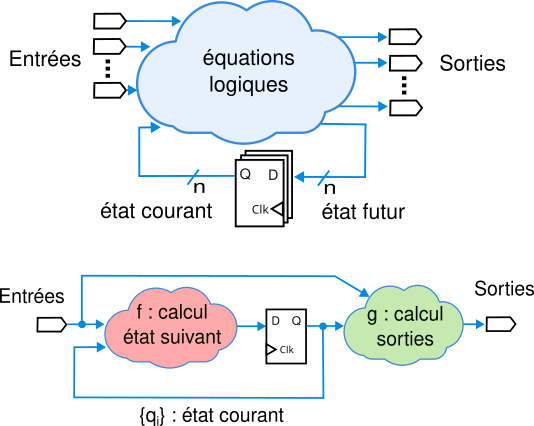
\includegraphics[scale=0.50]{./images/sys_0.png}

    \vspace{0.3cm}
    {\small Horloge implicite : le temps est discret, $t\in\mathbb{N}$.}
  \end{column}

  % ---------- Colonne droite : équations ----------
  \begin{column}{0.55\textwidth}
    \textbf{Bascule D :} $q(t+1) = d(t)$

    \medskip
    \textbf{Tout le circuit se ramène à :}
    \[
      \begin{cases}
        q_i(t+1) = d_i(t) = f_i\big(e(t),\,q(t)\big) & \text{(état suivant)}\\[2pt]
        s_j(t)   = g_j\big(e(t),\,q_j(t)\big) & \text{(sorties)}
      \end{cases}
    \]
    où $f_i,g_j$ sont des équations booléennes.

  \end{column}
\end{columns}

\end{frame}

%======================================================================
\begin{frame}{Systèmes séquentiels : schéma générique}
  \begin{columns}[T]
    % ---------- Colonne gauche : le circuit ----------
    \begin{column}{0.45\textwidth}
      \centering

      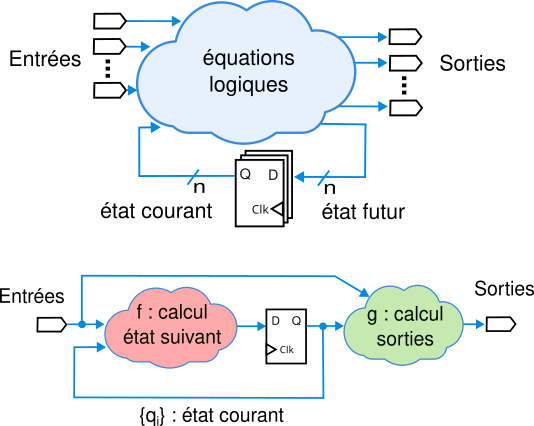
\includegraphics[scale=0.50]{./images/sys_0.png}

      \vspace{0.3cm}
      {\small Horloge implicite : le temps est discret, $t\in\mathbb{N}$.}
    \end{column}

    % ---------- Colonne droite : équations ----------

      \begin{column}{0.45\textwidth}
              \begin{block}{Analogie avec le monde continu}
                  \textbf{Monde continu (Physique/Syst. Dyn) :}
                  \[ \frac{d\mathbf{Q}}{dt} = \mathbf{f}(\mathbf{Q}, \mathbf{E}, t) \]
                  \vspace{0.2cm}
                  \textbf{Monde numérique (Discret) :}
                  \[ \mathbf{Q}_{t+1} = \mathcal{F}(\mathbf{Q}_t, \mathbf{E}_t) \]
                  \vspace{0.1cm}
                  \footnotesize L'horloge dicte le pas de temps : $dt \equiv T_{clk}$.
              \end{block}

              \begin{alertblock}{Le caractère \og exécutable \fg{}}
                  Contrairement aux équations différentielles sur le papier, le silicium \textbf{résout et exécute} ces équations en temps réel, front après front.
              \end{alertblock}
          \end{column}

  \end{columns}
\end{frame}
%======================================================================
\begin{frame}{Systèmes séquentiels : schéma générique et déclinaisons}
  \centering
  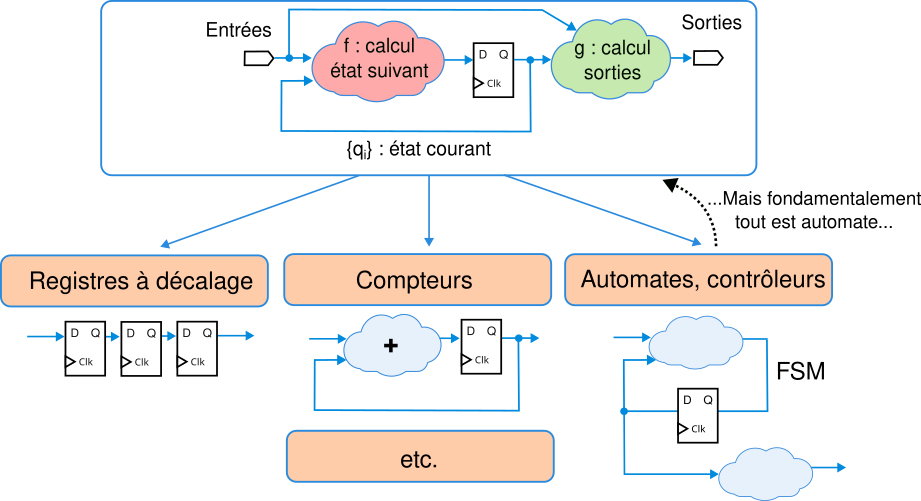
\includegraphics[scale=0.50]{./images/seq_3.png}

  \begin{center}
        \textbf{Conséquence :} Tout système dynamique discret, automate ou algorithme \\peut être \alert{matérialisé et simulé} par un réseau de bascules. \\
        \normalsize $\rightarrow$ \textit{Le circuit numérique possède un pouvoir de modélisation universel.}
    \end{center}
\end{frame}


\begin{frame}{Bascule D : Reset et Set \textit{asynchrones}}
\begin{columns}
  \begin{column}{0.45\textwidth}
    \begin{block}{Cas du \texttt{Reset} : mise à 0}
      \begin{itemize}
        \item Le \texttt{reset} est \textbf{prioritaire} sur l'horloge.
        \item Lorsqu'il est activé $\rightarrow Q=0$
      \end{itemize}
    \end{block}
    \begin{exampleblock}{Cas du \texttt{Set} : mise à 1}
      \begin{itemize}
        \item Le \texttt{set} est \textbf{prioritaire} sur l'horloge.
        \item Lorsqu'il est activé $\rightarrow Q=1$
      \end{itemize}
    \end{exampleblock}
    En cas d'ordres contradictoires $\rightarrow$ voire doc constructeur.

  \end{column}
  \begin{column}{0.45\textwidth}
    \centering
    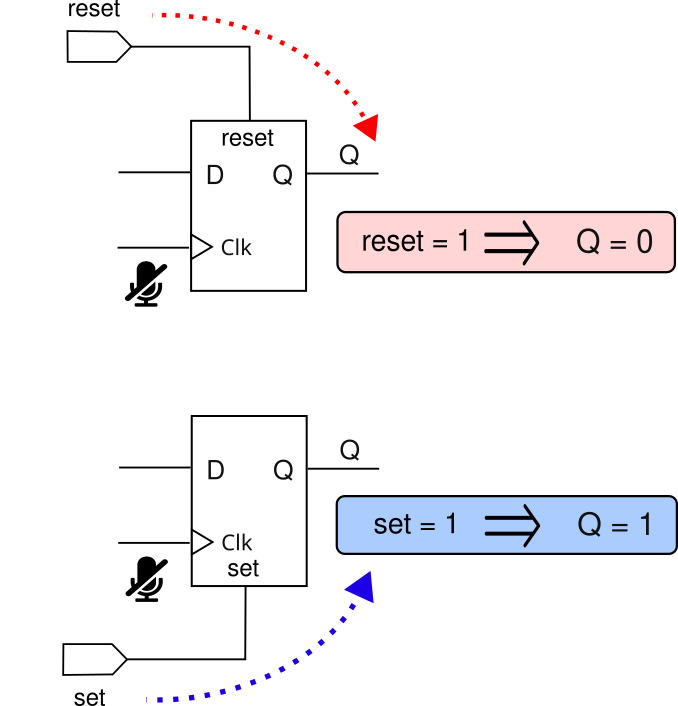
\includegraphics[scale=0.4]{./images/reset_0.png}
  \end{column}
\end{columns}
\end{frame}

\begin{frame}{Bascule D : Reset et Set \textit{asynchrones}}
\begin{columns}
  \begin{column}{0.40\textwidth}
    \centering
    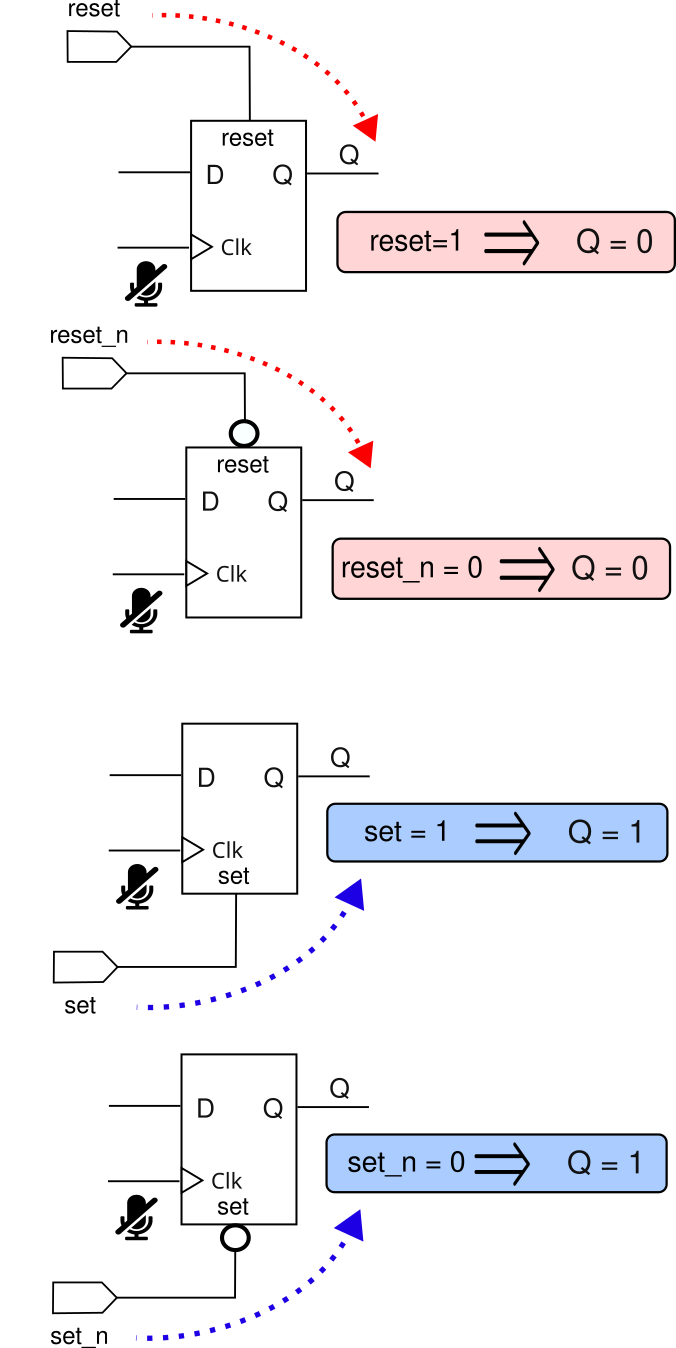
\includegraphics[scale=0.21]{./images/reset_1.png}
  \end{column}
  \begin{column}{0.55\textwidth}
    \begin{block}{Polarité d'activation}
      \begin{itemize}
        \item  Les deux signaux \texttt{reset} et \texttt{set} ont eux-mêmes une valeur où ils sont
        actifs.
        \item Cette valeur est précisée dans le schéma de la bascule :
        \begin{itemize}
          \item Cerle ° indique la \fbox{polarité \texttt{0} active}.
          \item L'\underline{absence de cercle} ° indique la \fbox{polarité \texttt{1} active}.
        \end{itemize}
        \item Cette valeur \textit{peut} être précisée dans le \textit{nommage} du signal :
        \begin{itemize}
          \item \texttt{reset\_n} indique une polarité \texttt{0} active.
          \item \texttt{reset} indique une polarité \texttt{1} active.
        \end{itemize}
      \end{itemize}
    \end{block}
    \begin{itemize}
      \item Les noms des signaux dépendent des \textit{conventions de nommage} propres aux entreprises.
      \item \textbf{Attention : } bien connecter \textbf{tous} les \texttt{reset} et \texttt{set}.
    \end{itemize}
  \end{column}
\end{columns}
\end{frame}
